% This file was created with tikzplotlib v0.10.1.
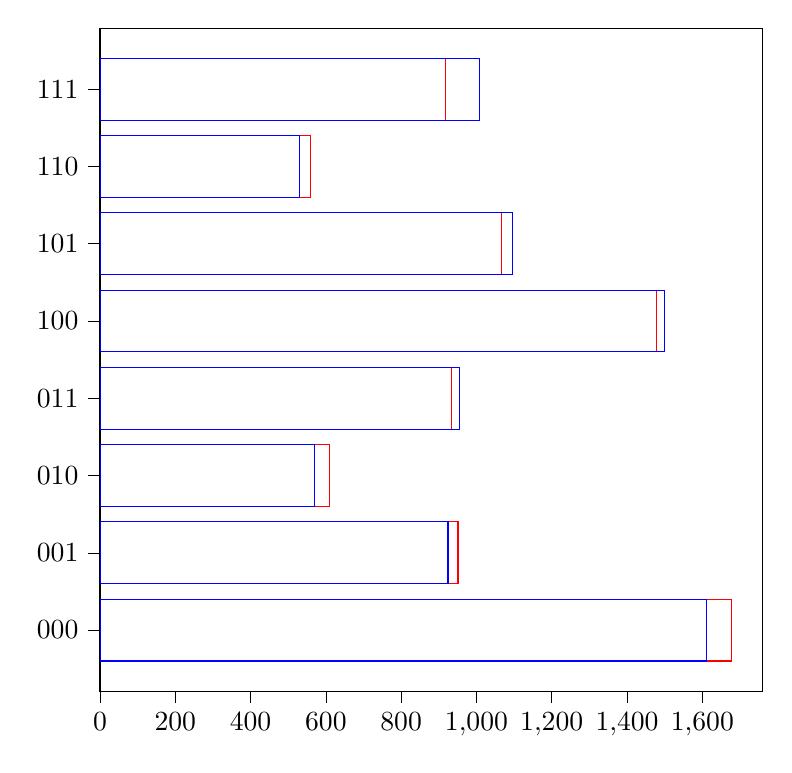
\begin{tikzpicture}

\definecolor{darkgray176}{RGB}{176,176,176}

\begin{axis}[
height=10cm,
tick align=outside,
tick pos=left,
width=10cm,
x grid style={darkgray176},
xmin=0, xmax=1760.85,
xtick style={color=black},
y grid style={darkgray176},
ymin=-0.79, ymax=7.79,
ytick style={color=black},
ytick={0,1,2,3,4,5,6,7},
yticklabels={000,001,010,011,100,101,110,111}
]
\draw[draw=red] (axis cs:0,-0.4) rectangle (axis cs:1677,0.4);
\draw[draw=red] (axis cs:0,0.6) rectangle (axis cs:951,1.4);
\draw[draw=red] (axis cs:0,1.6) rectangle (axis cs:609,2.4);
\draw[draw=red] (axis cs:0,2.6) rectangle (axis cs:933,3.4);
\draw[draw=red] (axis cs:0,3.6) rectangle (axis cs:1478,4.4);
\draw[draw=red] (axis cs:0,4.6) rectangle (axis cs:1067,5.4);
\draw[draw=red] (axis cs:0,5.6) rectangle (axis cs:560,6.4);
\draw[draw=red] (axis cs:0,6.6) rectangle (axis cs:917,7.4);
\draw[draw=blue] (axis cs:0,-0.4) rectangle (axis cs:1610.16679805322,0.4);
\draw[draw=blue] (axis cs:0,0.6) rectangle (axis cs:924.337419185712,1.4);
\draw[draw=blue] (axis cs:0,1.6) rectangle (axis cs:568.869911986052,2.4);
\draw[draw=blue] (axis cs:0,2.6) rectangle (axis cs:954.271867329141,3.4);
\draw[draw=blue] (axis cs:0,3.6) rectangle (axis cs:1500.07287394558,4.4);
\draw[draw=blue] (axis cs:0,4.6) rectangle (axis cs:1096.43617243261,5.4);
\draw[draw=blue] (axis cs:0,5.6) rectangle (axis cs:530.88817161411,6.4);
\draw[draw=blue] (axis cs:0,6.6) rectangle (axis cs:1006.95678545358,7.4);
\end{axis}

\end{tikzpicture}
